\chapter{Optical Enhancement of Core-Shell Nanowire} \label{data}

Given that the profound enhancement of optoeletronic properties of nanowires is
the major theme of this dissertation, it is dutiful to first summarize the
major experimental charateristics of Core-Shell nanowires (CSNWs)

Electron systems in lower dimensions are adequately treated through
perturbation methods. For 1D electron systems (1DES) the correlations among
electrons are much more significant due to higher degrees of confinement. The
electron can either be moving to the left or right and any small or localized
interaction can cause a collective response from the whole system. This is the
condition of broken symmetry, in which the overall status of the system has to
be reformulated. For a 2DES, a broken symmetry occurs at very low densityies of
fermions, in which formation of a Wigner lattice is expected, which is due to
the Coulombic interactions of electrons. Intererstingly for a 1DES, the
direction of movement for fermions is restricted to the left or right.
Consequently, the density of the sytem becomes irrelevant with respect to the
determination of the status of the system. Such a 1D many electron system is
often called a $L\ddot{u}finger$ Liquid, as he was the first person who
successfully formulated these systems.

Importantly, a 1DES can experimentally be realized in various material systems.
These include carbon nanotubes, electrons at the edges of a 2DES, and in
nanowires.

A core-shell nanowire (CSNW) is a quasi-one dimensional structure with a wide
band gap materials, such as AlGaAs, wrapping around a low band gap
semiconductor, such as GaAs.

It is expected that the lower dimensionality in CSNW to have a significant
influence on both optical and electrical properties of the structure. Fot
instantce,

Electrically it is important account for the electron correlations in order to
determine the behavior of the structure. The significant values ofr exchange
and correlation energies in 1DES. makes them an interesting candidate for
probing ther energy dynamics. This, however, imposes various experimental
challenges and theoretical considerations and are deferred to future
investigations.

\section{Growth of Nanowires}



\section{Scanning Electron Microscopy Images} 

Figure 1a is top view SEM image of nanowires of ~100nm diameter core of GaAs,
and ~40nm thick AlGaAs, with the inset showing a magnified image that
demonstrates the rather sparse distribution of the wires. Figure 1b shows the
reflectivity of a GaAs wafer on which 50nm thin film of AlGaAs is grown, and
compares this to the reflectivity spectrum of a Si substrate. As expected,
about 30% to 55% of a normally incident light is reflected in bulk Si and GaAs,
with a sharp change for wavelengths near their respective band gaps. Figure 1c
contrasts this with the measured absorption spectrum of two types of GaAs core,
AlGaAs shell (CS) nanowires (BW): those grown on a GaAs substrate (black), and
the others heteroepitaxially grown on a Si substrate (red). The spectra show
that both cases have the signature change of reflectivity at bandgap of GaAs,
i.e., these are due to the GaAs/AlGaAs CSNWs, not the substrate. Importantly,
for the wavelength range of 700-1200nm these core-shells which only occupy ~15%
of the volume compared to thin films of the same height, reflect 2-4% of light
for the CSNWs grown on Si, and 3-7% of light for those grown on GaAs substrate.
The beam-width of the incident light being ~1μm, this shows that only a few NWs
are interrogated by light and, normalized to volume, these wires absorb more
than two orders of magnitude more light than their thin-film counterparts.

\begin{figure}
  \caption{Scanning Electron Microscopy of Core-Shell Nanowire Grown on Si}
  \centering
  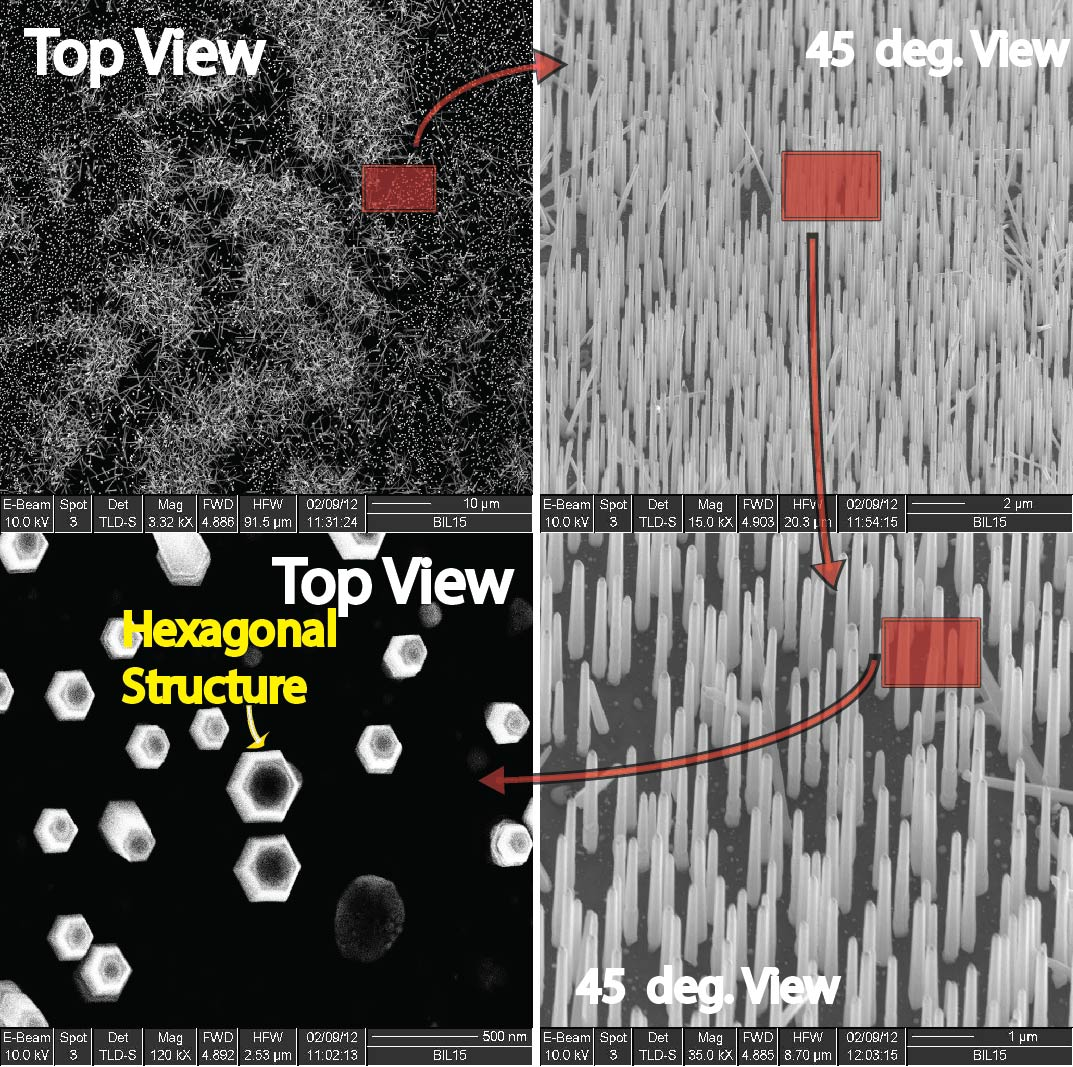
\includegraphics[width=\textwidth]{pictures/Data/SEMNW}
  \label{SEMNW}
\end{figure}

\section{Electrical Characterization of Nanowire}

\begin{figure}
  \caption{Current versus Voltage Measurment under illumination of Core-Shell Nanowire Grown on Si}
  \centering
  \includegraphics[width=\textwidth]{pictures/Data/CSNWIV_light}
  \label{CSNWIV_light}
\end{figure}

\section{Absorption Enhancement} \label{X-ray}

\begin{figure}
  \caption{Reflective Measurement for Bulk GaAs and Si}
  \centering
  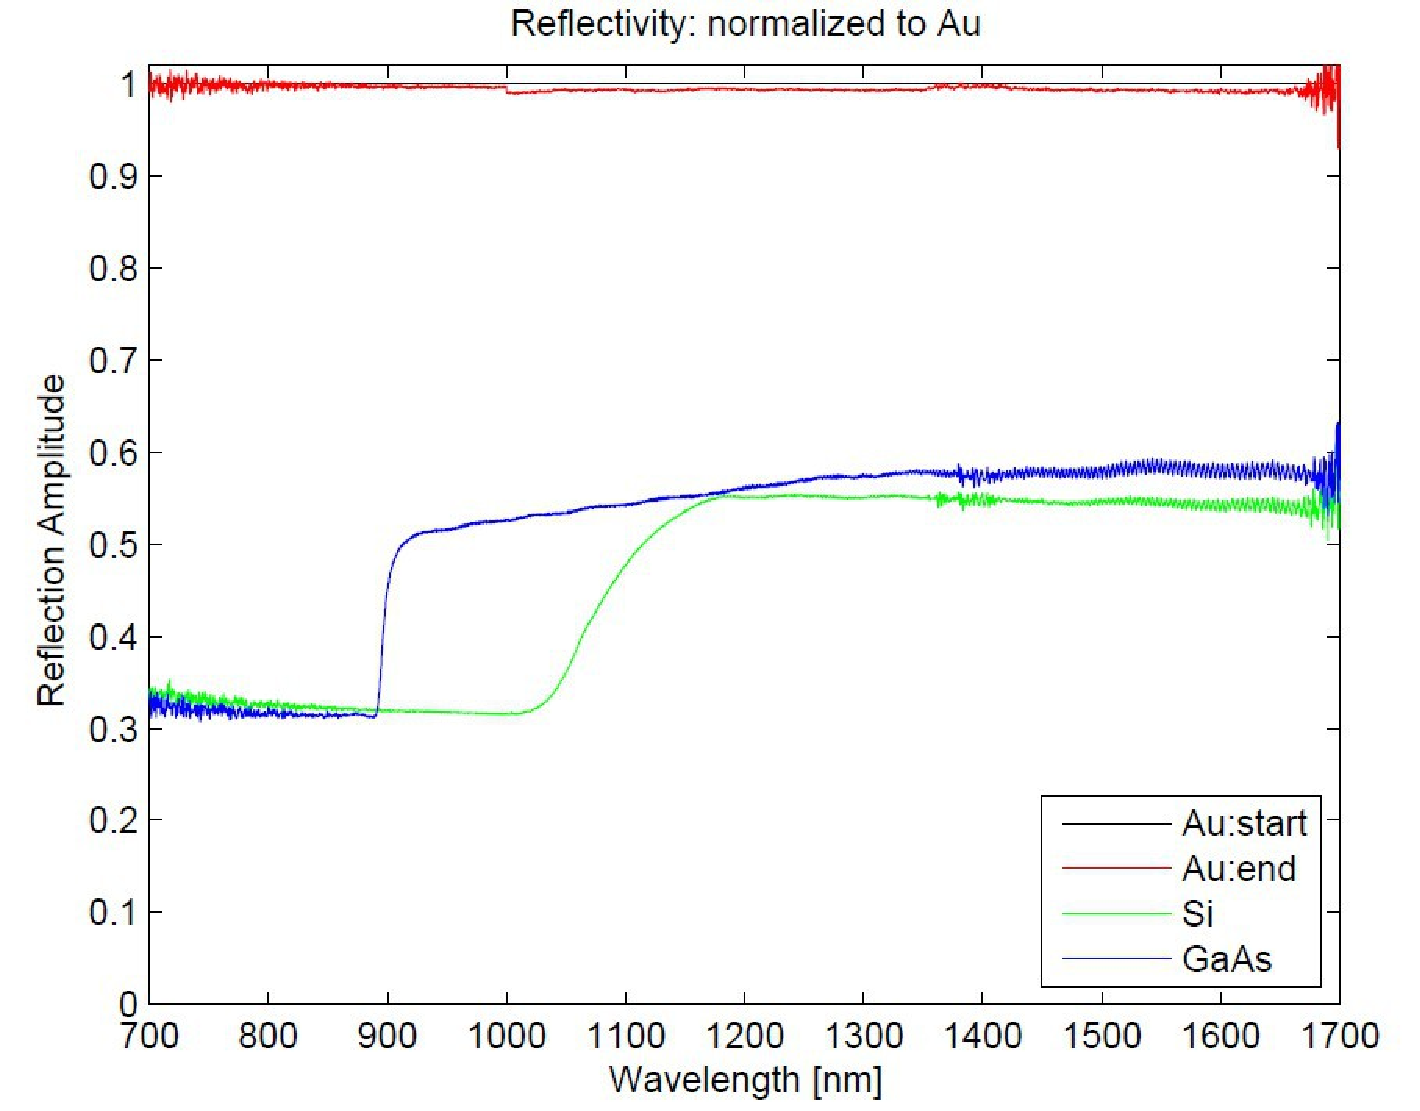
\includegraphics[width=\textwidth]{pictures/Data/reflecbulk}
  \label{reflecbulk}
\end{figure}

\begin{figure}
  \caption{Reflective Measurement for Core-Shell Nanowires Grown on Bulk GaAs and Si}
  \centering
  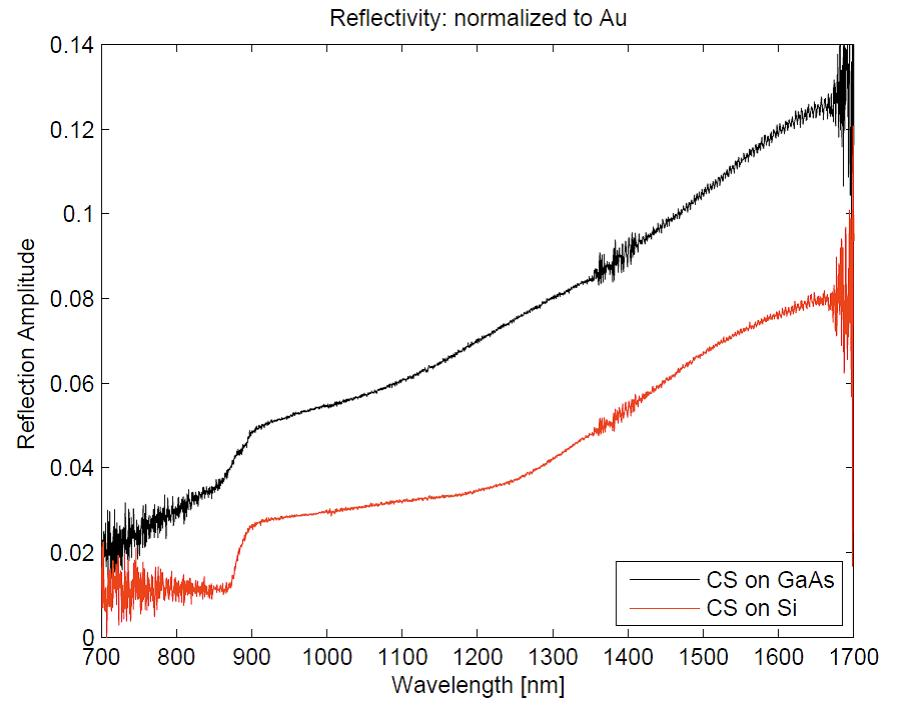
\includegraphics[width=\textwidth]{pictures/Data/reflectCSNW}
  \label{reflectCSNW}
\end{figure}

\section{Emission Enhancement} \label{Dust_data}

\begin{figure}
  \caption{Photoluminescence Experiment for Core-Shell Nanowires Grown on Bulk GaAs and Si}
  \centering
  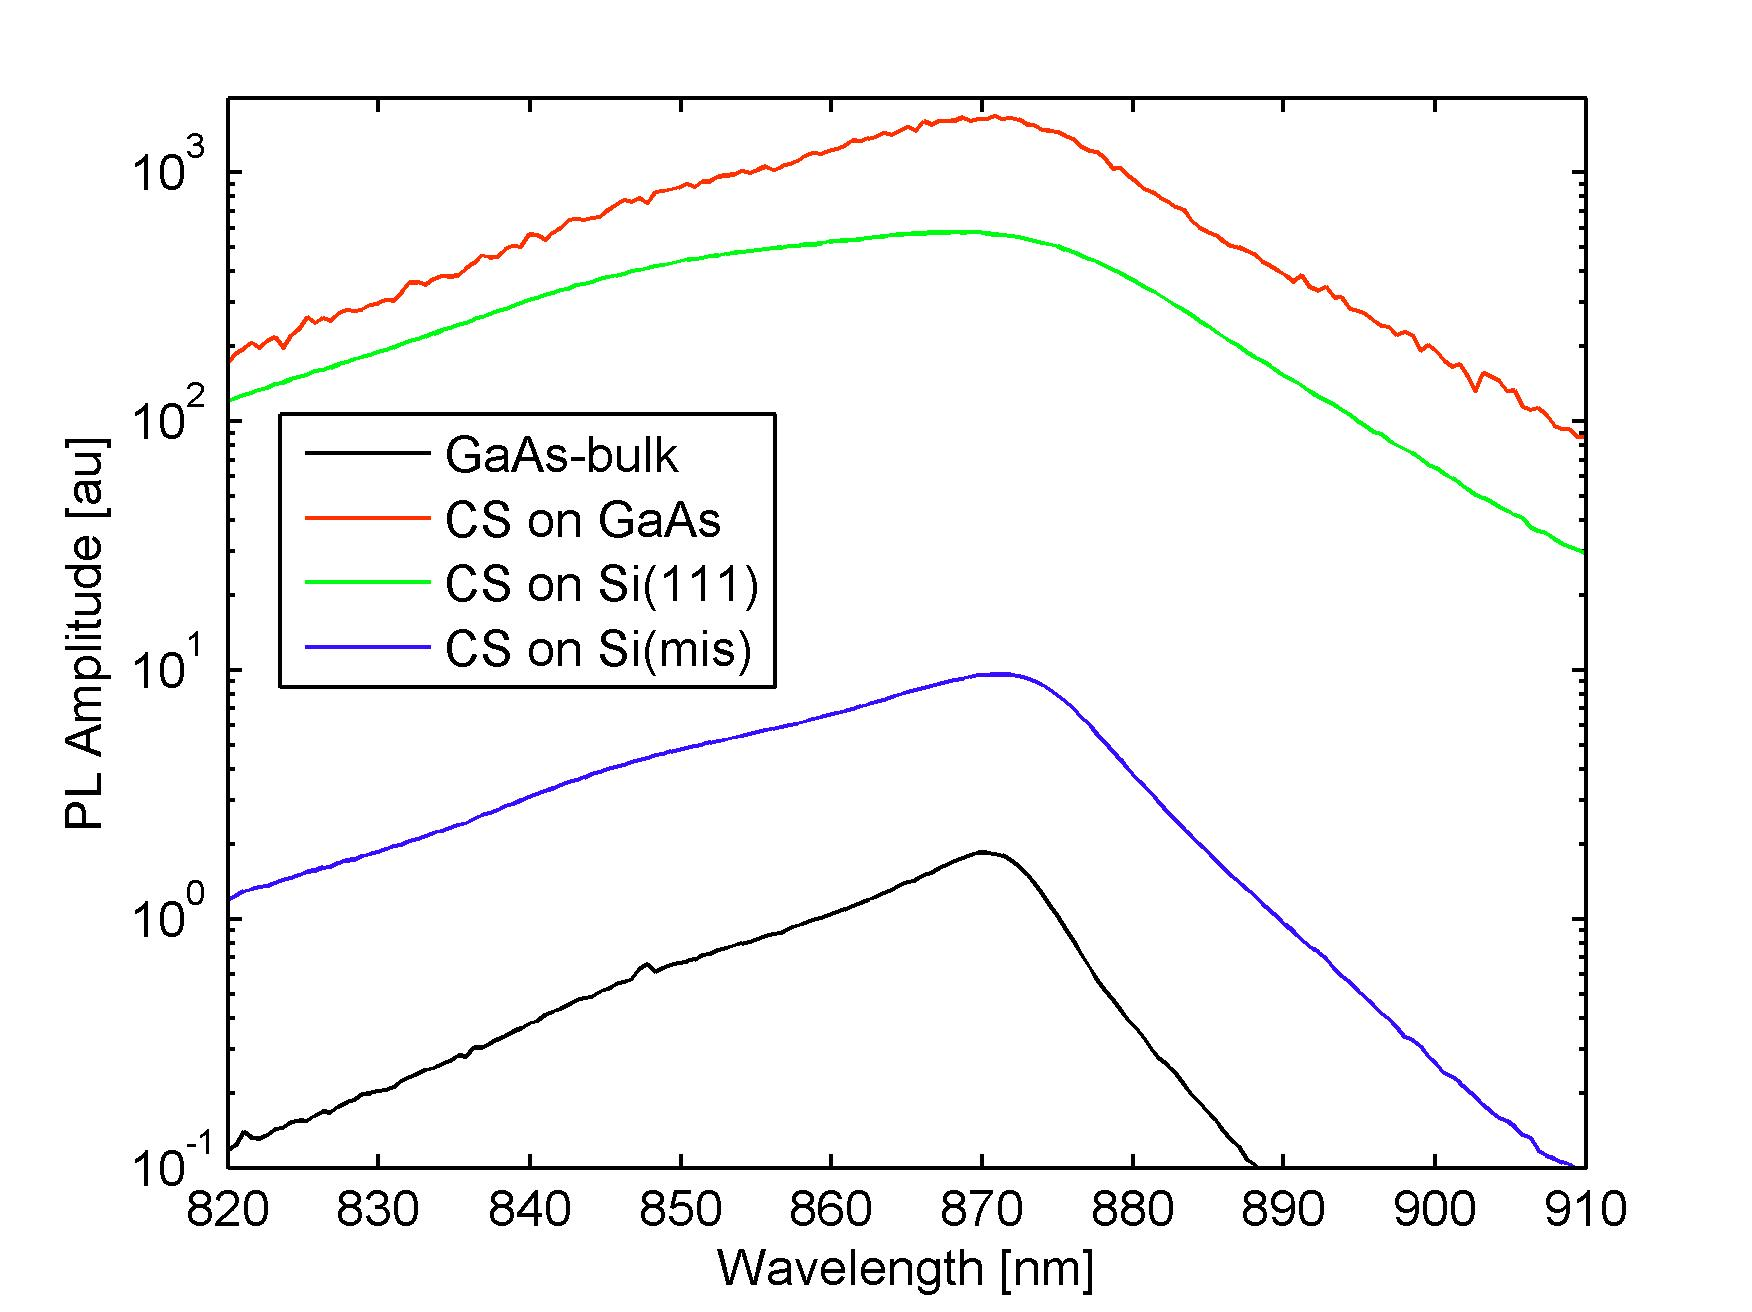
\includegraphics[width=\textwidth]{pictures/Data/PL}
  \label{PL}
\end{figure}

\section{Lasing} \label{BH_data}

\begin{figure}
  \caption{Photoluminescence Experiment Demonstrated Lasing Behavior for Core-Shell Nanowires Grown on Bulk GaAs and Si}
  \centering
  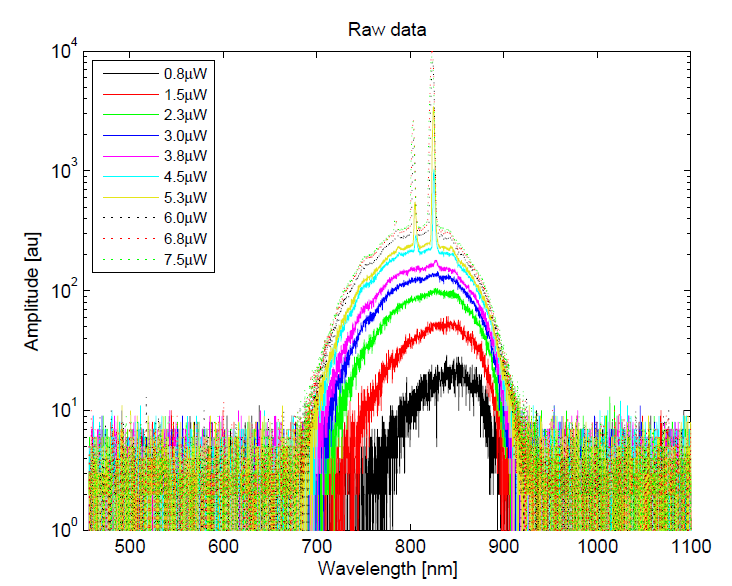
\includegraphics[width=\textwidth]{pictures/Data/lasing}
  \label{lasing}
\end{figure}
